% Created 2018-05-03 Thu 14:53
% Intended LaTeX compiler: pdflatex
\documentclass[final,12pt,a4paper]{article}

\usepackage{graphicx}
\usepackage{amssymb}
\usepackage[margin=0.5in]{geometry}
\usepackage{booktabs}
\usepackage{xcolor}
\usepackage{sourcecodepro}
\usepackage{url}
\usepackage{listings}
\usepackage[utf8]{inputenc}
\usepackage[english]{babel}
\usepackage{multirow}
\usepackage{textcomp}
\usepackage{caption}
\usepackage{hyperref}
\usepackage{sourcecodepro}
\usepackage{booktabs}
\usepackage{array}
\usepackage{listings}
\usepackage{graphicx}
\usepackage[english]{babel}
\usepackage[scale=2]{ccicons}
\usepackage{url}
\usepackage{relsize}
\usepackage{amsmath}
\usepackage{bm}
\usepackage{wasysym}
\usepackage{ragged2e}
\usepackage{textcomp}
\usepackage{pgfplots}
\usepgfplotslibrary{dateplot}
\setsansfont[BoldFont={Source Sans Pro Semibold},Numbers={OldStyle}]{Source Sans Pro}
\lstdefinelanguage{Julia}%
{morekeywords={abstract,struct,break,case,catch,const,continue,do,else,elseif,%
end,export,false,for,function,immutable,mutable,using,import,importall,if,in,%
macro,module,quote,return,switch,true,try,catch,type,typealias,%
while,<:,+,-,::,/},%
sensitive=true,%
alsoother={$},%
morecomment=[l]\#,%
morecomment=[n]{\#=}{=\#},%
morestring=[s]{"}{"},%
morestring=[m]{'}{'},%
}[keywords,comments,strings]%
\lstset{ %
backgroundcolor={},
basicstyle=\ttfamily\scriptsize,
breakatwhitespace=true,
breaklines=true,
captionpos=n,
commentstyle=\color{black},
extendedchars=true,
frame=n,
keywordstyle=\color{black},
language=R,
rulecolor=\color{black},
showspaces=false,
showstringspaces=false,
showtabs=false,
stepnumber=2,
stringstyle=\color{gray},
tabsize=2,
}
\renewcommand*{\UrlFont}{\ttfamily\smaller\relax}
\author{Pedro Bruel}
\date{\today}
\title{Autotuning: D-Optimal Designs}
\hypersetup{
 pdfauthor={Pedro Bruel},
 pdftitle={Autotuning: D-Optimal Designs},
 pdfkeywords={},
 pdfsubject={},
 pdfcreator={Emacs 25.3.1 (Org mode 9.1.12)}, 
 pdflang={English}}
\begin{document}

\maketitle
\tableofcontents


\section{Results}
\label{sec:orge42ea71}
\subsection{Comparing Strategies}
\label{sec:org8051c3e}
\begin{center}
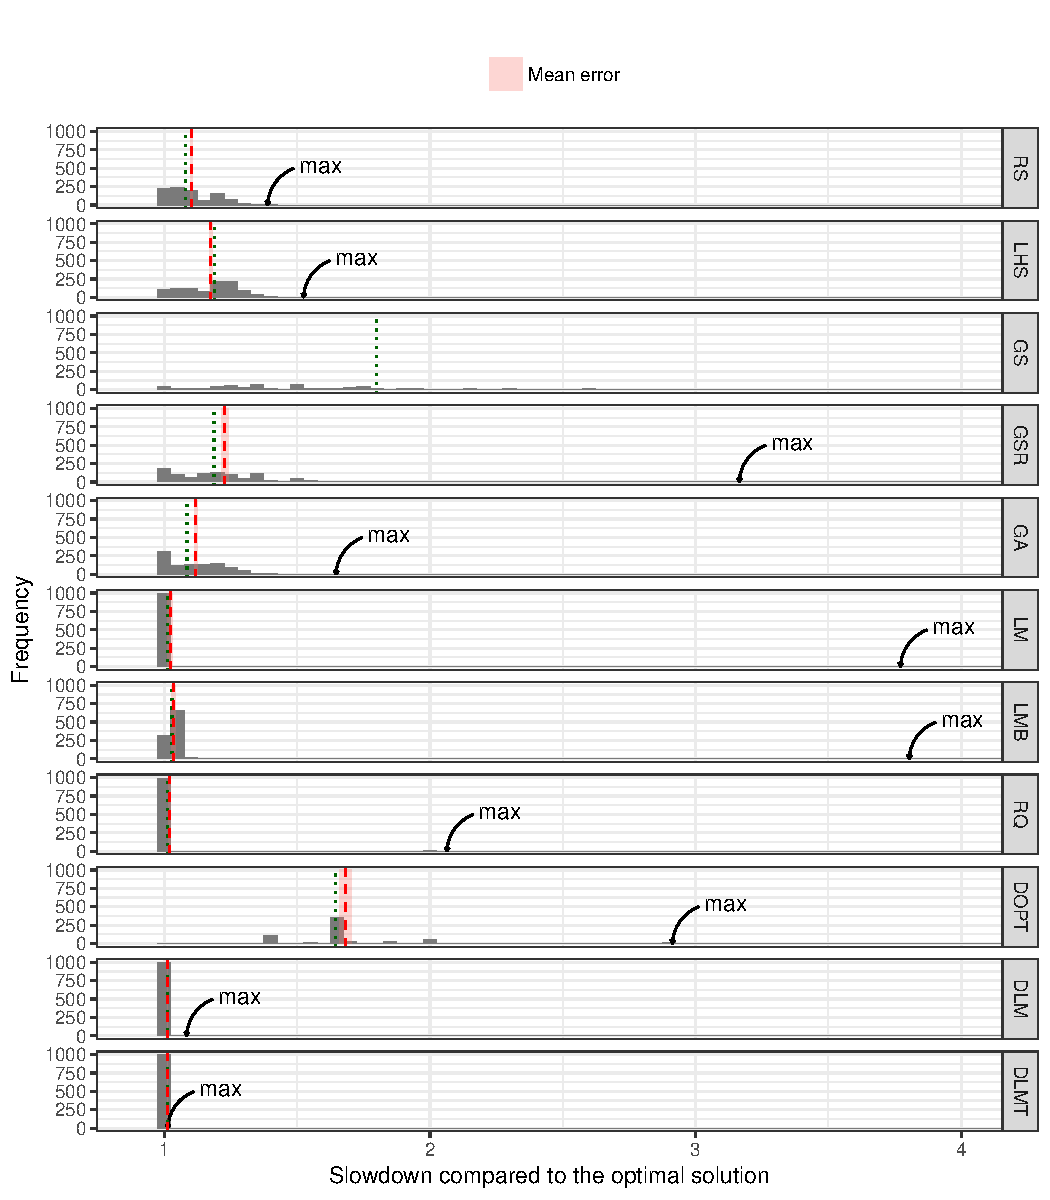
\includegraphics[width=.9\linewidth]{../img/comparison_histogram.pdf}
\end{center}

% latex table generated in R 3.4.4 by xtable 1.8-2 package
% Thu May  3 14:53:44 2018
\begin{table}[ht]
\centering
\begin{tabular}{lrrrrrrrrr}
  \hline
 & RS & LHS & GS & GSR & GA & LM & RQ & DOPT & DOPTaov \\ 
  \hline
Min. & 1.00 & 1.00 & 1.00 & 1.00 & 1.00 & 1.01 & 1.01 & 1.38 & 1.01 \\ 
  1st Qu. & 1.03 & 1.09 & 1.35 & 1.07 & 1.02 & 1.01 & 1.01 & 1.64 & 1.01 \\ 
  Median & 1.08 & 1.19 & 1.80 & 1.19 & 1.09 & 1.01 & 1.01 & 1.64 & 1.01 \\ 
  Mean & 1.10 & 1.17 & 6.46 & 1.23 & 1.12 & 1.02 & 1.02 & 1.68 & 1.01 \\ 
  3rd Qu. & 1.18 & 1.24 & 6.31 & 1.33 & 1.19 & 1.01 & 1.01 & 1.64 & 1.01 \\ 
  Max. & 1.39 & 1.52 & 124.76 & 3.16 & 1.65 & 3.77 & 2.06 & 2.91 & 1.08 \\ 
  Mean Pt. & 120.00 & 98.92 & 22.17 & 120.00 & 120.00 & 119.00 & 119.00 & 120.00 & 54.85 \\ 
   \hline
\end{tabular}
\caption{Summary statistics} 
\end{table}
\end{document}
